\chapter{Graphentheorie}
\section{Motivation}
Vieles vom Gesehenen sind Graphen.
\subsubsection{Hasse-Diagramme}
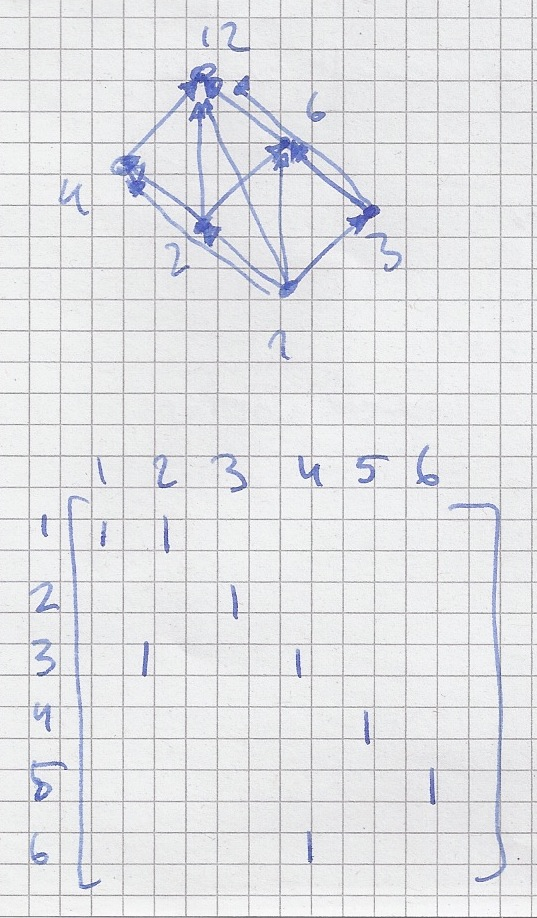
\includegraphics{Bild28} \\
Adjazenzmatrix des Graphen
\subsubsection{Relationen}
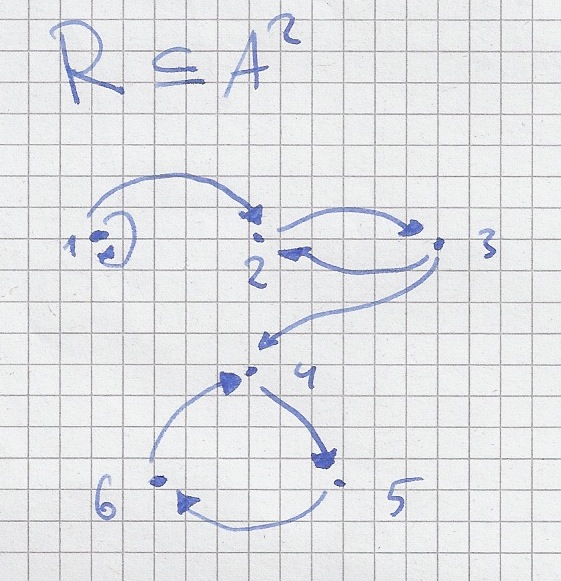
\includegraphics{Bild29} \\
\begin{bsp*}
	Gläser anstossen \\
	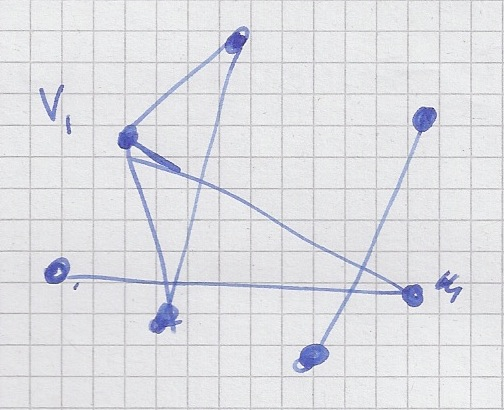
\includegraphics{Bild30} \\
	Anzahl derer, die mit ungerader Anz. anstossen, ist gerade.
	\begin{gather*}
		\deg(v_1) = 3 \\
		\sum_i \deg(v_i) = 2\underbrace{|E|}_{\substack{Anz.\\Kanten}} \\
		|\{i | \deg(v_i) \text{ ungerade}\}| \text{ gerade}
	\end{gather*}
\end{bsp*}
\begin{bsp*}[note = Fehlerfreie Kommunikation über verrauschte Kanäle]
	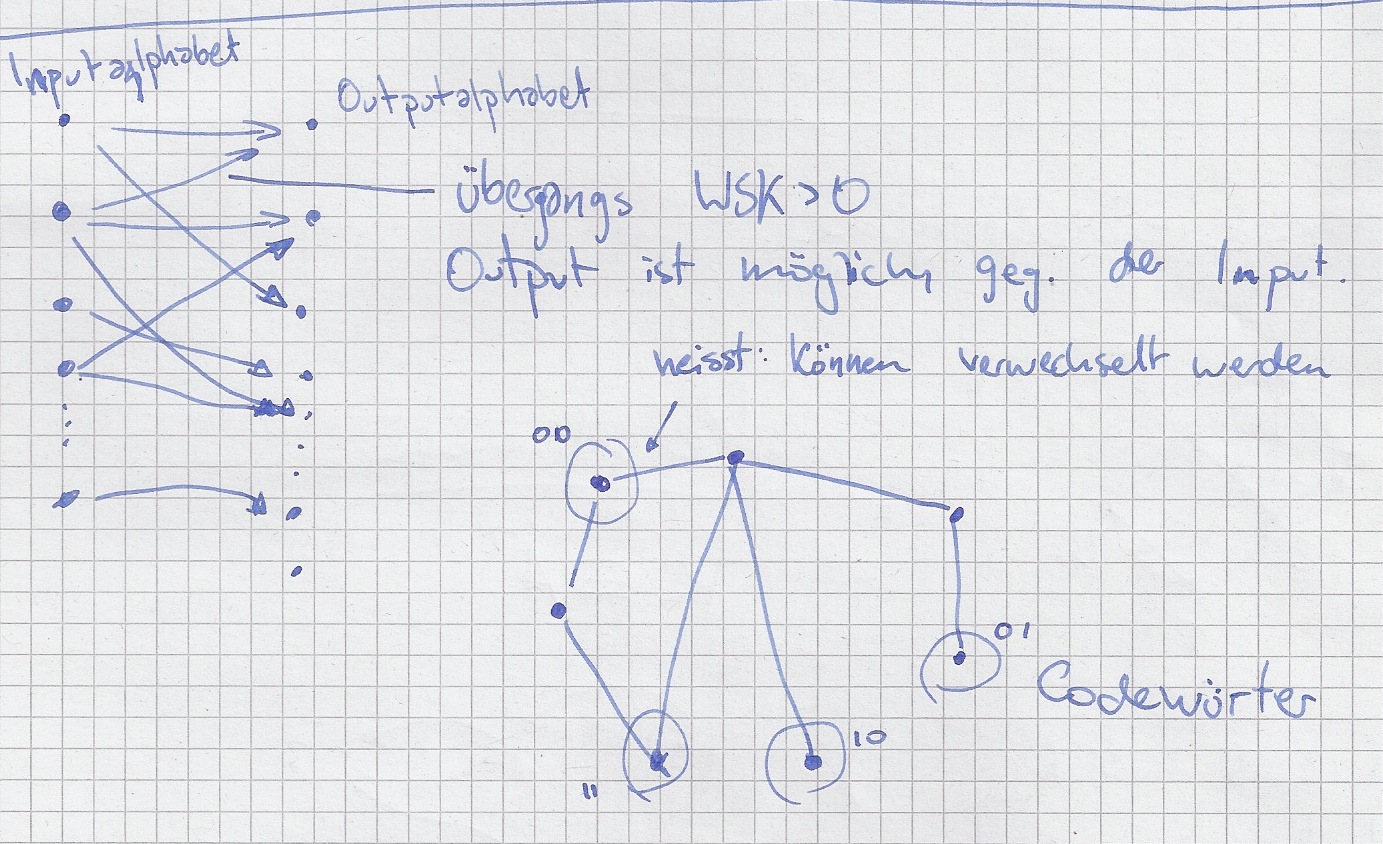
\includegraphics[width=\textwidth]{Bild31}
\end{bsp*}
\subsubsection{Konkreter Kanal(Shannon, 1948)}
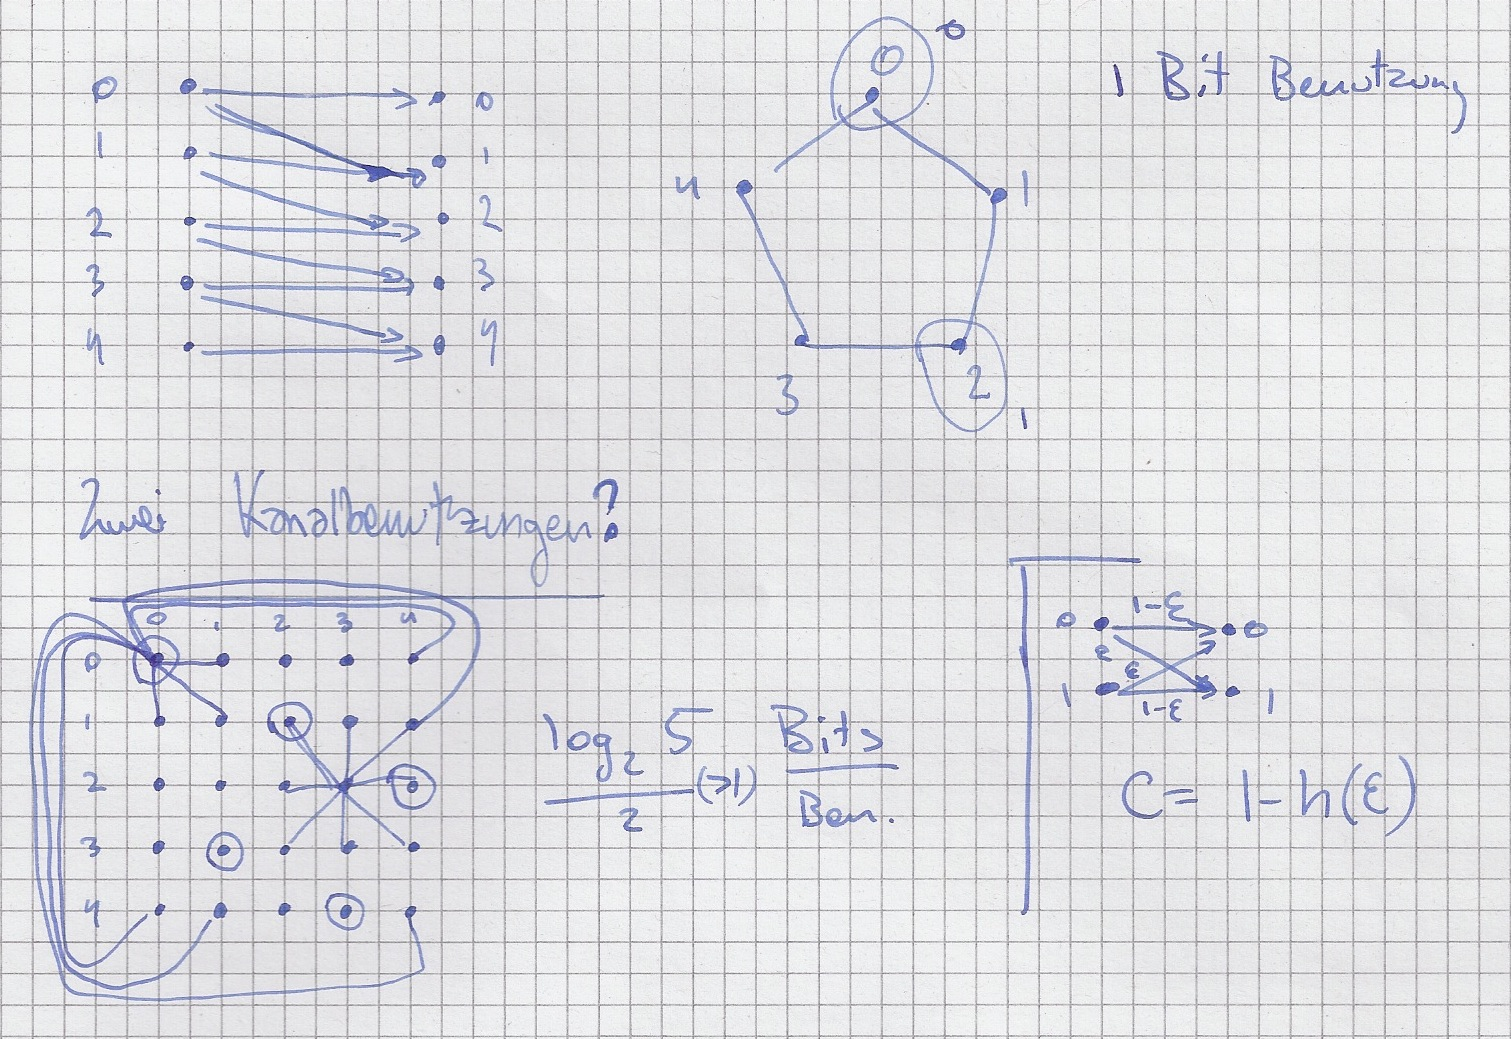
\includegraphics[width=\textwidth]{Bild32}
